\section{Literaturrecherche}
\label{sec:recherche} Für die Recherche zu den verschiedenen Teilaufgaben ist
die Dokumentation der Open Source Plattform 3D Slicer eine wichtige Ressource
\cite[vgl.]{[}]{slicer2024}. Diese zeigt bereits etablierte Verfahren und einen \textit{Best
Practise} Ansatz. Auch das \citet{extensionsIndex2024} Repository ist eine
wichtige Quelle, da so ein Einblick in andere Lösungen möglich ist. So kommt es,
das nach ausführlicher Recherche zu den Teilaufgaben UI-Design, Pseudo-Extension,
Kapselung Hoffmann, Speicherung Parameter, Dokumentation und Test bereits Lösungen
existieren. Bei diesen Lösungen handelt es sich jedoch nicht um konkrete
Ergebnisse, sondern vielmehr um einen Leitfaden zur Lösung der Teilaufgabe. Die
Recherche hat demnach ergeben, dass diese Teilprobleme im Kontext der 3D Slicer Umgebung,
nicht das erste Mal zutage treten und Lösungswege existieren.

\begin{minipage}{0.40\textwidth}
	Für ein \textbf{UI Design} wird sehr empfohlen, bereits etablierte 3D Slicer Extensions
	als Orientierung zu nutzen. Eine sehr gute Orientierung bietet das Modul
	\textit{Transforms}, das in Abbildung \ref{fig:module_example} zu sehen ist. Zu
	Erkennen ist, dass die UI mittels Collapsible Buttons in verschiedenen Gruppen
	unterteilt wird. Ohne in die verschiedenen Gruppen hineinzublicken, lässt sich
	gut abschätzen, welche Parameter wo zu erwarten sind. Dies ermöglicht dem
	Benutzer ein isoliertes Betrachten der unterschiedlichen Funktionen in diesem
	Modul und so eine gute Benutzerfreundlichkeit.
\end{minipage}
\hfill
\begin{minipage}{0.50\textwidth}
	\centering
	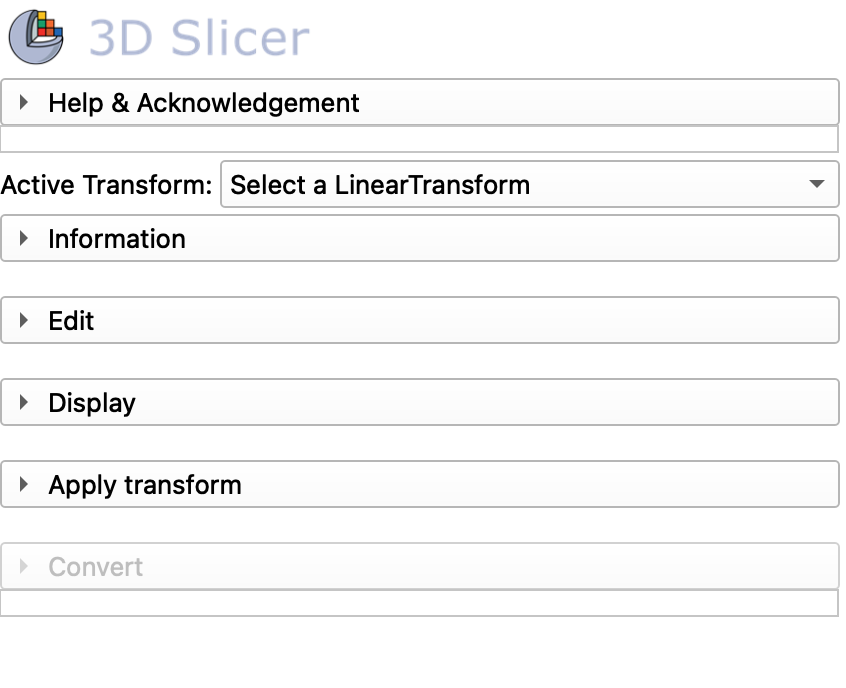
\includegraphics[scale=0.50]{img/modul_example.jpg}
	\captionof{figure}{Das Modul Transforms als Beispiel einer etablierten UI für eine Slicer Extension | Screenshot aus 3D Slicer}
	\label{fig:module_example}
\end{minipage}

Für die Extension, welche in der vorliegenden Arbeit erstellt werden soll, wird genau
dieser Ansatz gepflegt und somit eine gute Benutzbarkeit des Moduls gewährleistet.
Die speziellen wünsche der konkreten Benutzergruppe sollen jedoch nicht zu kurz
kommen.

Für das Erstellen einer \textbf{ersten funktionierenden Extension} bietet Slicer
eine sehr gute Hilfe. 3D Slicer hat hierfür ein eigenes Modul entwickelt, das sich
\textit{Extention Wizard} nennt. Dieses Modul gibt eine gute Einführung in die Entwicklung
mit Slicer. Hiermit lässt sich mittels Leitfaden eine erste Demo Extension
erstellen, die sich bereits gut in 3D Slicer einfügt. Diese Lösung könnte als
Abstraktionsschicht betrachtet werden, da durch dieses Modul im ersten Schritt nahe
zu keine Kenntnisse über die Kernanwendung von Slicer nötig sind. Der
Extentionwizard ist wie folgt zu finden:

\texttt{Modules -> Developer Tools -> Extension Wizard}

Für \textbf{die Kapselung} einer bestimmten Einheit von Code, sieht Slicer eine
Bibliothek innerhalb der Extention vor, so beschreibt es die \citet{slicer2024}.
Das Listing \ref{lst:3d_slicer_projektverzeichnis} zeigt, wo eine Bibliothek
innerhalb einer Extention einzuordnen ist, hier als \texttt{MyLib} zu sehen. Innerhalb
dieses Ordners können sich weitere Module befinden, die als einfache Python-Files
abgelegt werden. Zu beachten ist, dass in jeder Bibliothek eine \texttt{\_\_init\_\_.py}
hinzugefügt wird, sodass dieser Ordner auch entsprechend verwendet werden kann.

\begin{lstlisting}[
    language={python},
    caption={Prinzipeller Aufbau eines Projektes für eine Slicer Extension nach Slicer (2024)},
    label={lst:3d_slicer_projektverzeichnis}]
|-- CMakeLists.txt
|-- MyLib
|   |-- __init__.py
|   |-- cool_maths.py
|   |-- utils.py
|-- MyExtension.py
\end{lstlisting}

Für die Teilaufgabe zur \textbf{Speicherung der Parameter} nutzt Slicer eine
Technik, das durchaus als eines der Kernfunktionen beschrieben werden kann. Die
Rede ist hier von der Klasse \texttt{ParameterNodeWrapper}. Dieser wurde bereits
zu einem früheren Zeitpunkt in dieser Arbeit beschrieben. Für die Funktion dieser
Lösung sei auf den Abschnitt \ref{subsec:benutzerschnitstelle} Benutzerschnittstelle
verwiesen.

Sowohl das \textbf{Benutzerhandbuch}, also auch die technische Dokumentation einer
Slicer Extension wird immer in der \texttt{README.md} des jeweiligen Repository
hinterlegt. In der Extension selber sieht Slicer keine umfangreiche Dokumentation
vor. Es wird lediglich via Link auf die Dokumentation im Repository verwiesen
und eine kurze Einführung gegeben. Auch hier gibt es wieder etablierte Designs,
die als Vorlage verwenden werden können. Die \citet{slicer2024} erwähnt hier
unter anderem das Module
\href{https://github.com/lassoan/SlicerSegmentMesher}{SegmentMesher} als gutes
Beispiel.

Für die letzte Teilaufgabe, das \textbf{Testen}, gibt die Dokumentation von 3D Slicer
ebenfalls eine konkrete Struktur vor. Ist also nicht nötig eigenen Verfahren zu
entwickeln. Für die Softwaretests stell Slicer eine eigene Klasse innerhalb der Slicer
Bibliothek bereit, die alle wichtigen Funktionen enthält, um konkrete Testfälle zu
schreiben. Die Klasse trägt den Namen \textsl{ScriptedLoadableModuleTest} und kann
als Elternklasse für einen Testfall verwendet werden.

\begin{lstlisting}[
    language={python},
    caption={Aufbau einer Testklasse zum ausführen von Unittest nach \citet{slicer2024}},
    label={lst:3d_slicer_test_class}]
class MyExtensionTest(ScriptedLoadableModuleTest)
    def setUp(self):
      # do something befor a test
    def runTest(self):
      # execute your test case here
    def testMyExtension1(self):
      # write your test case here
\end{lstlisting}

Im Listing \ref{lst:3d_slicer_test_class} ist zu sehen, dass sich die Klasse in drei
Teil aufteilt, die Methode \texttt{setUp()}, die als Vorbedingung dient, die Methode
\texttt{runTest()}, die über die UI getriggert werden kann, um die Test zu
starten und die konkreten Textfälle, die in selbst definierten Methoden geschrieben
werden können. Als Beispiel sie hier die Methode \texttt{testMyExtension1()} gezeigt.

Im Laufe dieses Kapitels wurde klar, dass es für einige der Teilaufgaben bereits
Lösungen oder Lösungsansätze gibt, die zu etwas weniger Entwicklungsarbeit führen.
Jedoch trifft dies nicht auf alle Punkte zu, sodass sich der nächste Abschnitt mit
der Erarbeitung von konkreten Lösungsansätzen für die noch nicht behandelten Teilaufgaben
beschäftigt.
% ---------------------------------------------------------------------------------------

\section{Erarbeiten von Lösungsansätzen}
\label{sec:lösungsansätze} hier geht es um Brainstorming

\textbf{Architekturdesign}

\textbf{Single Prozess}

\textbf{Batch Prozess}

% ---------------------------------------------------------------------------------------
\subsection{Benutzerschnittstelle}
\label{subsec:benutzerschnitstelle} Für das Erstellen einer \ac{UI}, die für
eine Slicer Erweiterung notwendig ist, nutzt 3D Slicer den Qt-Designer \citep[vgl.][]{qt2024}.
Die Integration des Qt-Designers als Applikation in eine andere Applikation funktioniert
aufgrund der Plattformintegrität, die der Designer mitbringt \citep[vgl.][]{qt2024}.
Diese bietet so die Möglichkeit die benötigten Widgets über eine interaktive
Benutzerschnittstelle zu bauen. Für diese \ac{UI}-Vorrichtung gibt es einen
Gegenspieler im Quelltext des Programmes, welcher als \textit{ParameterNode}
bekannt ist. Der \textit{ParameterNode} ist laut \citet{slicer2024} eine leichte
Variante eines \ac{MRML}-Knoten um Parametereinstellungen zu speichern. Durch das
Zusammenspiel zwischen \ac{UI} und \textit{ParameterNode} wird die \ac{UI}
automatisch aktualisiert, wenn sich das Programm ändert \citep[vgl.][]{slicer2024}.

\begin{minipage}{0.35\textwidth}
	Das Erstellen der Verknüpfung zwischen \ac{UI}-Widget und \textit{ParameterNode}
	erfolgt über die dynamische Eigenschaft \texttt{SlicerParameterName}, die direkt
	in der Komponentenansicht im Qt-Designer einstellbar ist. Die Abbildung
	\ref{fig:qt_designer} soll diesen Vorgang verdeutlichen. Dabei ist es wichtig,
	dass genau diese Eigenschaft auch verwendet wird. Diese Verknüpfung lässt sich
	laut \citet{slicer2024} auch via Programmcode setzten.
\end{minipage}
\hfill
\begin{minipage}{0.55\textwidth}
	\centering
	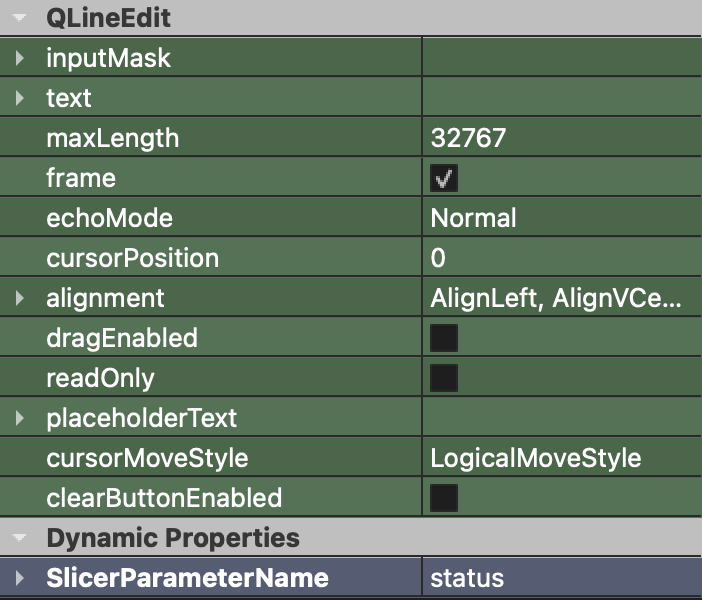
\includegraphics[width=0.5\textwidth]{img/qt_designer.png}
	\captionof{figure}{Komponentenansicht im Qt-Designer nach der \citet{slicer2024}}
	\label{fig:qt_designer}
\end{minipage}

Über das Objekt \texttt{widget} kann die Eigenschaft einer Komponente gesetzt
werden, ohne dass sie im Designer berührt werden muss. Das nachfolgende Beispiel
zeigt dies genauer.
\begin{center}
	\texttt{widget.setProperty('SlicerParameterName', 'parameterName')}
\end{center}
Mit dem Ende dieses Abschnittes wurden alle wichtigen Bestandteile von 3D Slicer
abgedeckt und diskutiert, sowie alle weiteren Domänen eingeführt. So bleibt nun die
Frage nach dem Sinn dieser Arbeit. Das Kapitel \ref{chap:fragestellung} soll
hier Klarheit liefern und die konkrete Fragestellung ausarbeiten.
% ---------------------------------------------------------------------------------------

\chapter{Einleitung}
\label{chap:einleitung} Die \ac{CT} hat die Medizintechnik revolutioniert und
ist bis heute eines der wichtigsten Methoden für die Bildanalyse. Sie ist eine der
führenden Erweiterungen der klassischen Röntgentechnik. Für die Entwicklung
dieser Technologie wurden Godfrey Newbold Hounsfield und Allan McLeod Cormack im
Jahre 1979 mit dem Nobelpreis für Medizin ausgezeichnet \citep[.vgl][S.~12]{handels2000}.

\begin{minipage}{0.45\textwidth}
	Die Computertomografie wird in den verschiedensten Bereichen und im wahrsten Sinne
	des Wortes von Kopf bis Fuß eingesetzt. So kommt es, dass auch im Dentalbereich
	\ac{CT}-Aufnahmen von größter Wichtigkeit sind. Abbildung \ref{fig:ct_aufnahme_eines_zahns}
	zeigt eine solche \ac{CT}-Aufnahmen. Eine konkrete Anwendung in diesem Kontext
	ist die Zahnkaries Forschung der Poliklinik für Zahnerhaltung und Parodontologie
	der \ac{LMU}.
\end{minipage}
\hfill
\begin{minipage}{0.45\textwidth}
	\centering
	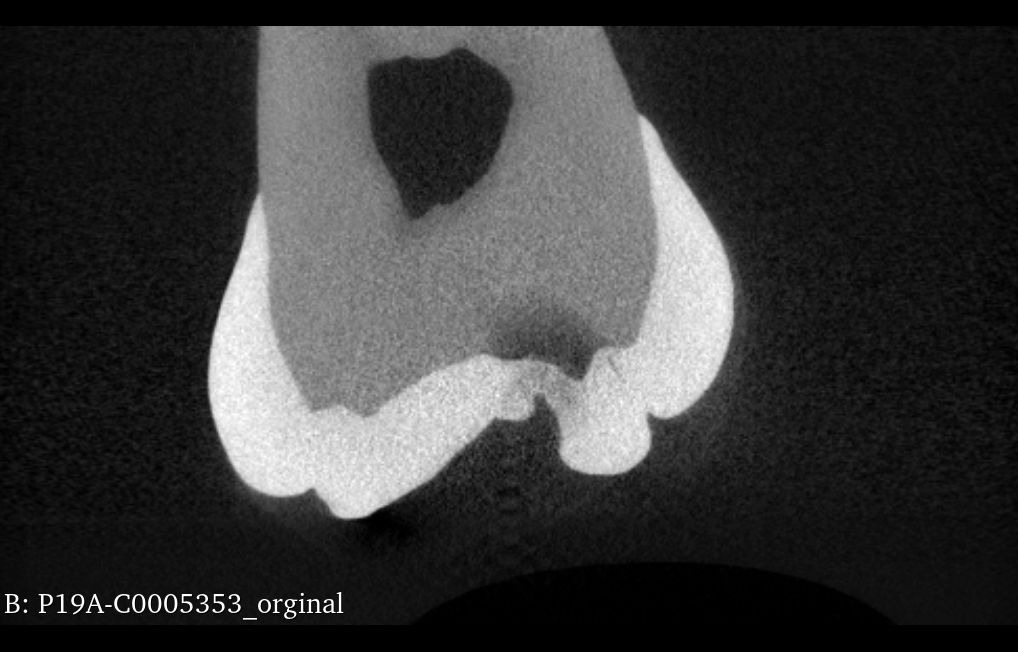
\includegraphics[scale=0.2, width=\textwidth]{img/micro_ct_orginal.jpg}
	\captionof{figure}{CT-Aufnahme eines Zahns nach \citet{heck2024}} \label{fig:ct_aufnahme_eines_zahns}
\end{minipage}

Die vorliegende Arbeit soll genau diese Forschung unterstützen. In welchem Umfang
und zu welchem Grund ist in den folgenden Abschnitten beschrieben.
% ---------------------------------------------------------------------------------------

\section{Ziel der Arbeit}
\label{sec:ziel_der_arbeit} Diese Arbeit beschreibt eine Technik, mit der \ac{3D}
Mikro-\ac{CT}-Bilder zur Untersuchung zahnmedizinischen Strukturen automatisch
mittels der Software 3D Slicer segmentiert und analysiert werden können. Was genau
unter eine Segmentierung verstanden wird, darüber informiert das Kapitel
\ref{subsec:segmentierung} Segmentierung. Die algorithmische Formulierung einer konkreten
Segmentierung ist bereits vorhanden und prototypisch implementiert. Dieser
Algorithmus hat jedoch Schwachstellen. So muss beispielsweise das Verfahren umständlich
über ein IPython Notebook im Terminal ausgeführt werden, was die
Benutzerfreundlichkeit deutlich beeinträchtigt. Ziel dieser Arbeit ist es in erster
Linie das bereits existierende Verfahren in der Klinik für Zahnerhaltung zu analysieren
und für die Mitarbeiter der Klinik benutzbar zu machen. Dabei soll auf
etablierte und vertraute Lösungen zurückgegriffen werden.

Es stellt sich nun die Frage, zu welchem Zweck eine automatische und interaktive
Segmentierung überhaupt notwendig ist. Für die Zahnklinik an der LMU in München
gibt es hierfür viele Gründe. Über den wichtigsten gibt das nächste Kapitel Aufschluss.
% ---------------------------------------------------------------------------------------

\section{Relevanz der Arbeit}
\label{sec:relevanz_der_arbeit} Der wohl relevanteste Punkt wurde bereits im vorherigen
Kapitel \ref{sec:ziel_der_arbeit} diskutiert, Zahnärzte sind keine
Softwareentwickler, sondern reine Anwender von Software. Darüber hinaus verfolgt
die Klinik für Zahnerhaltung und Parodontologie der \ac{LMU} einen sehr interessanten
Forschungsansatz, welche eine Segmentbetrachtung der \ac{CT}s rechtfertigt.

Über viele Jahre hinweg wurden in der Zahnklinik sehr viel Bilddaten von Zähnen
gesammelt. Hierbei wurden Aufnahmen der unterschiedlichsten Arten gemacht.
Darunter fallen zum Beispiel einfache Bilddateien, Infrarotbilder und die für diese
Arbeit so relevanten dreidimensionalen Mikro-CT-Aufnahmen. Dieser große Schatz
an Bildmaterial soll verwendet werden, um in ferner Zukunft ein neuronales Netzwerk
zu trainieren, welches statistische Aussagen über das Verhalten von Karies
treffen kann. Jedoch gibt es hier ein Problem, bei dem das Ergebnis dieser
Arbeit unterstützen kann. Karies auf \ac{CT}-Bildern zu lokalisieren ist nicht
trivial. Er ist ohne weitere Bearbeitung des Bildes nur sehr schwer auf eine Stelle
einzugrenzen. So kommt es vor, dass drei verschiedene Ärzte auf demselben Mikro-\ac{CT}-Bild
drei unterschiedliche Stellen mit Karies identifizieren. Eine Segmentierung des dreidimensionalen
\ac{CT}s kann hier Wunder wirken. Durch die Aufteilung des Mikro-\ac{CT}s in
seine zwei Zahnhauptsubstanzen, kann eine sehr gute visuelle Darstellung des Zahnes
gewährleistet werden. Für Ärzte bietet diese Darstellung einen sehr großen
Mehrwert \citep[vgl.][S.~1]{walter2025projekt}.

Mit dieser klaren und eindeutigen Identifizierung von Karies, sind die
Ergebnisse, die ein neuronales Netzer generieren würde viel genauer und brauchbarer.
Konkret wird mit einer automatischen Segmentierung ein \textit{Ground Trueth} gewonnen,
der eine eindeutige Basiswahrheit liefert. Hierbei sei gesagt das diese Anwendung
nur eine von vielen Möglichkeiten ist. Konkrete Daten über die Ausbreitung einer
Krankheit im menschlichen Körper zu besitzen kann in den verschiedensten Fällen
und Institutionen von größtem Nutzen sein. So zeigen es auch \citet[S.~207]{de20083d}
in ihrem Paper.

Anhand dieser Argumente wird deutlich, dass eine automatische Segmentierung durchaus
einen Mehrwert für Ärzte bilden kann. Nicht zuletzt auch durch die enorme
Zeiteinsparung. Für eine automatische Segmentierung von Mikro-\ac{CT}-Bildern
gibt es einige Softwarelösungen am Markt, die alle eine gute Optionen sind. Aus
diesem Grund soll im folgenden Kapitel ein mögliches Framework diskutiert werden.
% ---------------------------------------------------------------------------------------

\section{Fokus der Arbeit}
\label{sec:fokus_der-arbeit} Dieser Arbeit setzt den Fokus auf die Open-Sorce-Plattform
3D Slicer, da diese ohnehin bereits eine breite Anwendung in der Zahnklinik in München
findet. Durch die Modul- und Plug-in-Infrastruktur dieser Plattform kann die Software
auch anderen Institutionen bereitgestellt werden. Hierzu muss diese einfach als
\textit{3D Slicer Extension} bereitgestellt werden. 3D Slicer bietet einen
\textit{Extension Manager}, der ähnlich wie ein App Store betrachtet werden kann.
So bleibt die vorerst konkret entwickelte Software nicht nur einer Einrichtung vorbehalten.
Eine tiefere Einführung in die Open-Source-Plattform bietet der Abschnitt
\ref{sec:3d_slicer}. Das weitere Optimieren des bereits bestehenden Verfahrens wird
in dieser Arbeit nicht thematisiert. Es werden lediglich Anpassungen vorgenommen,
sodass eine Benutzerschnittstelle verwendet werden kann.

Mit diesem Umfang, der Motivation und dem gesetzten Fokus, ergibt sich für diese
Arbeit eine konkrete Struktur, die einen hohen Detailgrad aufweist. Um einen ersten
Überblick zu gewähren, sei diese Struktur hier kurz erläutert.
% ---------------------------------------------------------------------------------------

\section{Aufbau der Arbeit}
\label{sec:aufbau_der_arbeit} Die Arbeit ist in sieben Kapitel unterteilt. Nach der
Einführung in Kapitel \ref{chap:einleitung}, in der die Relevanz und der Fokus
beschrieben werden, werden in Kapitel \ref{chap:theoretische_grundlagen} die theoretischen
und technischen Grundlagen behandelt, welche zum Verstehen der Ergebnisse
essenziell sind. Als Ergebnis der theoretischen Grundlagen bildet das Kapitel \ref{chap:fragestellung}
eine konkrete Forschungsfrage. Während sich Kapitel \ref{chap:methodik} darum
kümmert mit welchen Methodiken und Lösungsansätzen an die Forschungsfrage
herangegangen wird, erläutert das Kapitel \ref{chap:ergebnisse} welche die konkreten
Ergebnisse der Arbeit sind. In Kapitel \ref{chap:diskussion} erfolgt eine
kritische Diskussion der Resultate. Das abschließende Kapitel \ref{chap:schlussfolgerung}
fasst die wichtigsten Erkenntnisse zusammen und gibt einen Ausblick auf zukünftige
Forschungsfragen.

Die theoretischen Grundlagen, die wie beschrieben direkt nach der Einleitung
folgen, sind zentral für das Verstehen der Fragestellung und der späteren Ergebnisse
der Arbeit.
% ---------------------------------------------------------------------------------------

\section{Anatomische Segmentierung von Mikro-CT-Bildern}
\label{sec:verwwandte_arbeit} Wie bereits in der Einleitung dieser Arbeit klar wurde
verfügt die Poliklinik für Zahnerhaltung und Parodontologie des \ac{LMU}-Klinikums
München über einen breiten Schatz an Bilddaten. Im Rahmen einer Bachelorarbeit an
der Hochschule für angewandte Wissenschaften in Augsburg unterstützte Herr Hofmann
die Verarbeitung dieser Bilddaten mit Methoden der 3D-Bildverarbeitung. Konkret
sollte diese Arbeit die Kariesklassifizierung unterstützen. Hierzu entwickelte er
ein Verfahren, das auf Basis adaptiver Schwellwertverfahren die Zahnsubstanzen
Schmelz und Dentin aus dem Originalbild herauslöst. Konkret kann diese Segmentierung
mit verschiedenen Verfahren durchgeführt werden. Man spricht hier von einer
anatomischen Segmentierung der Zahnkrone.

\begin{minipage}{0.40\textwidth}
	Durch die Segmentbetrachtung der beiden Zahnhauptteile Schmelz und Dentin konnte
	\citet[S.~41]{hoffmann2020} eine gute Hilfe für die Befundung kariöse Stellen
	liefern. Ein Ergebnis aus der Arbeit von Hofmann sei in Abbildung \ref{fig:ergebnis_hoffmann}
	gezeigt. \citet[S.~53]{hoffmann2020} entwickelte hierfür ein prototypisches Verfahren,
	mit dem es gelang ca. 250 Datensätze der Zahnklinik automatisch aufzubereiten.
\end{minipage}
\hfill
\begin{minipage}{0.50\textwidth}
	\centering
	
\includegraphics[width=0.7\textwidth]{img/ergebnis_hoffmann_2.jpg}
	\captionof{figure}{Reproduzierte Ergebnisansicht der anatomischen Segmentierung}
	\label{fig:ergebnis_hoffmann}
\end{minipage}

Die anatomische Segmentierung des Zahnes umfasst eine ganze Reihe algorithmischer
Schritte, sodass sich eine Pipeline an Verarbeitungsschritten ergibt. Die Abbildung
\ref{fig:anatomische_segmentierung} zeigt den groben Ablauf des Verfahrens.
Kleinere Zwischenschritte wurden nicht berücksichtigt.

\begin{figure}[h]
	\centering
	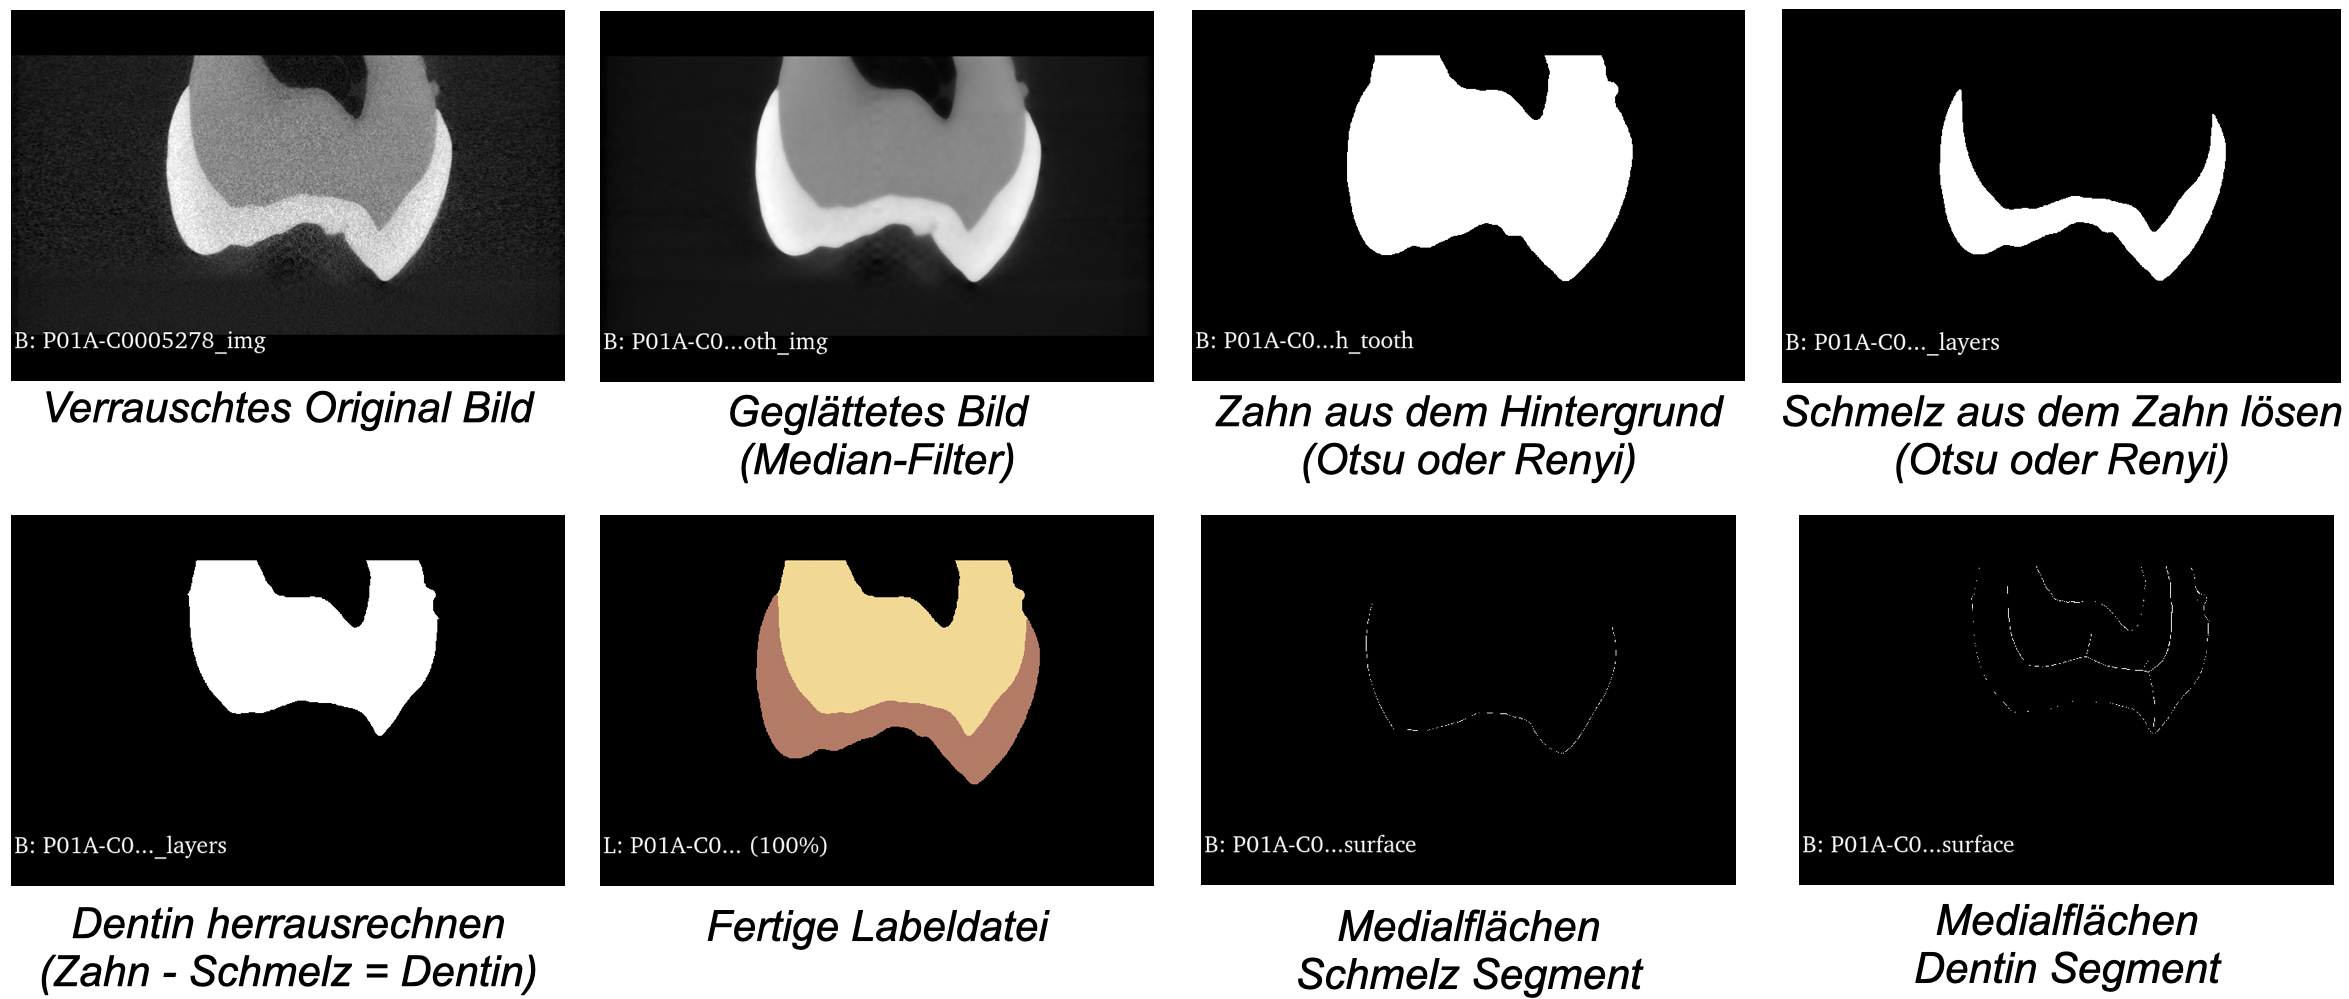
\includegraphics[width=0.8\textwidth]{img/anatomischeSegmentierung.png}
	\caption{Algorithmische Formulierung der anatomischen Segmentierung nach
	\citet{hoffmann2020}}
	\label{fig:anatomische_segmentierung}
\end{figure}

\citet[S.~55]{hoffmann2020} beschreibt, dass dieses Verfahren bis zu einem gewissen
Fortschritt des Karies durchgeführt werden konnte, da der Algorithmus
diesbezüglich seine Grenzen hat. Außerdem ist das Verfahren für die ordinalen \ac{ISQ}-Bilder
erstellt worden, deren Daten im Format \ac{16Int} vorliegen. Für die spätere Darstellung
der Ergebnisse kann eine überlappende Ansicht in einer Visualisierungssoftware verwendet
werden. So ergibt sich die Situation, dass der Algorithmus ein gutes Ergebnis liefert,
jedoch nicht benutzerfreundlich zu bedienen ist. Für das Starten und visualisieren
des Verfahrens sind aufwendige Befehle über das Terminal zu tippen \citep[vgl.][S.~53]{hoffmann2020}.
Genau an dieser Stelle soll die vorliegende Arbeit anknüpfen und das Verfahren der
anatomischen Segmentierung so interaktiv und benutzerfreundlich gestalten.

Für eine interaktive Verarbeitung von 3D Bilddaten bieten sich einige Möglichkeiten.
Die wohl beste Lösung liefert 3D Slicer. Warum die Wahl auf diese Plattform fiel
und welche Vorteile daraus entstehen wird im folgenden Abschnitt \ref{sec:3d_slicer}
erläutert.
% ---------------------------------------------------------------------------------------

\subsection{Datenformate}
\label{subsec:datensätze} Die rohen Datensätze, welche direkt aus dem Mikro-\ac{CT}-Gerät
kommen, haben nach \citet{scanco2024} das Format \ac{ISQ}. Dieses Format fällt speziell
auf die Geräte der Firma SCANCO zurück. Wie das vorherige Kapitel
\ref{subsec:computertomografie} bereits eingeführt hat, ist dieser Dateityp für eine
weitere Bearbeitung nur bedingt geeignet. Unter anderem wegen ihrer Größe. \citet[S.~118-119]{RoeschKunzelmann2018}
haben hierfür ein Paket entwickelt. Dieses konvertiert ein \ac{ISQ} Format in
ein \ac{MHD} Format. Bei einer \ac{MHD}-Datei handelt es sich um ein Metafile,
dass auf die eigentliche Datei verweist. Folgender Ausschnitt zeigt die Verwendung
des Pakets.
\begin{center}
	\texttt{python3 isq\_to\_mhd.py <quelle> <ziel>}
\end{center}
Diese Metadatei kann genutzt werden, um interessante Informationen über das Bild
zu erlangen. Wird dieses Kommando ausgeführt, so erstellt das Skript \texttt{isq\_to\_mhd}
ein Metafile, das detaillierte Daten über die Datei enthält. Ein Ausschnitt
dieses Metafiles liefer das Listing \ref{lst:inhalt_mhd_datei}

\begin{lstlisting}[
	caption={Ausschnitt des Inhaltes einer MHD-Datei},
	label={lst:inhalt_mhd_datei}]
ObjectType = Image
NDims = 3
CenterOfRotation = 0 0 0
ElementSpacing = 0.02 0.02 0.02
DimSize = 1024 1024 517
ElementType = MET_SHORT
ElementDataFile = P01A-C0005278.ISQ
\end{lstlisting}

In der Datei sind Informationen über die Ausprägung, Art und Größe der Datei zu finden.
Besonders interessant sind die Punkte \texttt{DimSize und ElementType}. Über
diese Parameter lässt sich die Größe eines Bildes berechnen. \citet[S.~10-11]{burger2009}
erklärt, dass ein Bild in Zellen aufgeteilt ist, welche Informationen enthalten.
Diese Zellen sind im zweidimensionalen Raum als Pixel bekannt. Betrachtet man
jedoch ein, wie im Falle der Zahnklinik an der \ac{LMU} dreidimensionales Bild, so
spricht man nicht mehr von einem Pixel, sondern von einem Voxel. Ein Voxel ist demnach
das dreidimensionale Äquivalent zu einem Pixel. \citet[S.~10-11]{burger2009} beschreiben
weiter das jeder diese Zellen ein binäres Wort der Länge $2^{k}$ ist. Die Basis
2 ergibt sich durch das binäre Wort, wo hingegen für $k$ gilt:
$k \in \mathbb{N}$. Um für den konkreten Fall aus Listing \ref{lst:inhalt_mhd_datei}
das entsprechenden $k$ zu ermitteln, muss der \texttt{ElementType} näher betrachtet
werden. \texttt{MET\_SHORT} steht hierbei für \textit{Signed short}, was eine Größe
von 16 Bit entspricht. Damit ergibt sich für die Länge $k$ ein Wert von 4. So
können nach \citet[S.~10-11]{burger2009} folgende Gleichungen festgehalten werden.

\begin{align}
	\label{equ:größe_bestimmen}1024 \cdot 1024 \cdot 517    & = 542,113,792 \, \text{Voxel}\notag  \\
	542,113,792 \, \text{Voxel}\cdot 2 \, \text{Byte/Voxel} & = 1,084,227,584 \, \text{Byte}\notag \\
	1,084,227,584 / 1,000,000,000                           & = 1.0842 \, \text{GB}
\end{align}

Die erste Gleichung bestimmt die Gesamtzahl aller Voxel in einem Bild. Gleichung
zwei ermittelt die Größe des Bildes in der Einheit Byte. Die letzte Zeile nimmt
eine Umrechnung von Byte nach \ac{GB} vor.

Durch die Gleichungen in \ref{equ:größe_bestimmen} wird klar, dass eine \ac{CT}-Aufnahme
des Typs \ac{ISQ} direkt nach seiner Aufnahme über einen \ac{GB} groß ist. Es
stellt sich also die spannende Frage, wie solch eine Datei komprimiert werden kann,
ohne das es Verluste in der Qualität gibt. Dr. Elisa Walter hat hierfür eine
Lösung entwickelt. Betrachtet man den \texttt{ElementType} genauer, so fällt auf,
dass es noch weitere Typen gibt, die durch eine geringere Länge $k$ deutlich weniger
Speicher benötigen. Durch Anwendung simpler Statistik lässt sich herauslesen, dass
die $2^{4}$ Byte je Element nicht ausgenutzt werden. Als Werkzeug für die
Betrachtung einer solchen Statistik kann das Histogramm eines Bildes genutzt
werden. Laut \citet[S.~249]{jahne2024} ist ein Histogramm die
Häufigkeitsverteilung der Grauwerte. Diese zeigt grafisch die unterschiedlichen Grauwerte
(x-Achse) zu ihren Häufigkeiten im Bild (y-Achse). \citet[S.~249]{jahne2024} macht
deutlich, dass das Histogramm jedoch kein Aufschluss über die räumliche
Verteilung der Pixel oder Voxel liefert. Werden einige der Argumente nicht verwenden,
so kann der \texttt{ElementType} verkleinert werden.
% ---------------------------------------------------------------------------------------

\textbf{Das Verfahren nach Rényi} ist ein weiteres Verfahren, das im Laufe dieser
Arbeit noch eine wichtige Rolle spielt. Wie bereits beschrieben gehört es
ebenfalls zu der Gruppe der Schwellwertverfahren und generiert demnach einen
Schwellwert $t$. Wie auch das Verfahren nach Otsu, benötigt Rényi keine
Information über die räumliche Anordnung der Bilder, es genügt das Bildhistogramm.
Dabei ist der optimal Schwellwert $t$ der, der eine maximale Entropie der Bildverteilung
erzeugt. Unter einer Entropie wird ein Konzept verstanden, das eine Unordnung,
Unsicherheit oder den Informationsgehalt innerhalb eines Systems beschreibt, so \citet[S.~102]{bein2006}.
Die Rényi-Entropie ist eine Verallgemeinerung der Shannon-Entropie und hängt von
einem Parameter $q$ ab. Die Entropie misst die Unsicherheit oder den
Informationsgehalt einer Wahrscheinlichkeitsverteilung, welche sich wie folgt ausdrücken
lässt. \citep[vgl.][K.~2]{bromiley2004}.

\begin{align}
	\label{equ:renyi}H_{q}(P) = \frac{1}{1-q}\ln \left( \sum_{i=1}^{N}p_{i}^{q}\right)
\end{align}

Besonderes Augenmerk verdienen hierbei die Parameter $p_{i}$ und $q$, welche die
charakteristischen Eigenschaften der Rényi-Entropie beschreiben. Der Parameter
$p_{i}$ ist die Wahrscheinlichkeit eines jeden Grauwertes im Bild. $i$ symbolisiert
hierbei jeden Grauwert. Wie viele Grauwerte genau betrachten werden sollen
definiert $N$. Die Variable $q$ hingegen beeinflusst die Gewichtung der Wahrscheinlichkeit
$p_{i}$ für jeden Grauwert. Setzt man den Parameter $q$ auf $q = 1$ so lässt
sich mittels Algebra die Shannon-Entropie zeigen \citep[vgl.][K.~2]{bromiley2004}.
Um nun mit der Rényi-Entropie den optimalen Schwellwert für ein Bild zu
berechnen, sieht Rényi ähnlich wie Otsu eine Einteilung in Klassen vor. Die
Einteilung erfolgt mittels des Parameters $N$. So kann nun für jede gebildete Klasse
die Gleichung \ref{equ:renyi} angewendet werden. Die Gesamtentropie des Systems
wird aus den beiden Teilentropien der jeweiligen Klassen bestimmt\citep[vgl.][K.~2]{bromiley2004}.
\begin{align}
	H_{q}(T) = H_{q}(P)^{(1)}+ H_{q}(P)^{(2)}
\end{align}
Um nun den optimalen Schwellwert $t$ bestimmen zu können muss der Wert genommen werden,
bei dem die Gesamtentropie des Systems maximal ist. Dieser Sachverhalt lässt sich
wie folgt ausdrücken \citep[vgl.][K.~2]{bromiley2004}.
\begin{align}
	t = max(H_{q}(T))
\end{align}
Neben unzähligen weiteren Segmentierungstechniken, ist eine für diese Arbeit von
ganz besonderer Bedeutung. Diese Technik wurde speziell zum Segmentieren der Mikro-\ac{CT}-Bilder
des Zahnklinikums an der \ac{LMU} in München entwickelt.

\pagebreak
% ---------------------------------------------------------------------------------------

\chapter{Forschungsfrage}
\label{chap:fragestellung} Dieses Kapitel beleuchtet die zentrale Frage, welche
mit Hilfe der Ergebnisse dieser Arbeit beantwortet werden soll. Dabei kann die Fragestellung
in erster Linie als Ergebnis der theoretischen Grundlagen aus Kapitel \ref{chap:theoretische_grundlagen}
interpretiert werden.

Die vorliegende Arbeit befasst sich mit der Erstellung einer Erweiterung für die
Plattform 3D Slicer, die ein spezifisches Segmentierungsverfahren auf Basis der
anatomischen Segmentierung integriert. Die Grundlagen für diese Methode bildet das
Kapitel \ref{sec:verwwandte_arbeit}. Die anatomische Segmentierung nutzt
bestehende Segmentierungsmethoden und wurde speziell für die Anforderungen der
Zahnklinik in München entwickelt. Sie ist prototypisch implementiert und zeigt in
ihrer Funktionalität vielversprechende Ergebnisse. Allerdings hat das aktuelle
Verfahren eine wesentliche Einschränkung: Es muss über das Terminal ausgeführt werden.
Dies erschwert die Anwendung in der klinischen Praxis und reduziert die
Benutzerfreundlichkeit erheblich. Als interaktive Lösung bietet sich die Software
3D Slicer an, da sie bereits in der Zahnklinik eingesetzt wird und über eine
flexible Infrastruktur für die Integration von Erweiterungen verfügt. Diese Eigenschaften
machen Slicer zu einer idealen Plattform, um die anatomische Segmentierung der
Zahnkronen in einer benutzerfreundlichen Form bereitzustellen.

Die zentrale Frage, die so aus den Grundlagen abgeleitet werden kann, teilt sich
in drei einzelne Fragen auf, die hier zu sehen sind.

\begin{description}
	\item[1. Fragestellung] kann das Verfahren der anatomischen Segmentierung als \ac{SEM}
		in Slicer implementiert werden?

	\item[2. Fragestellung] ist es möglich, die Integration so zu gestalten, dass der
		zugrunde liegende Algorithmus problemlos austauschbar ist oder zusätzliche Algorithmen
		eingebaut werden können?

	\item[3. Fragestellung] welche Erfahrungen lassen sich bei der Entwicklung einer
		Slicer-Extension sammeln, und welche Herausforderungen treten dabei auf?
\end{description}

Im folgenden Kapitel wird dargestellt, wie diese Fragestellung methodisch bearbeitet
wurde. Es wird gezeigt, wie das Problem strukturiert in Teilaufgaben zerlegt wurde
und welche Schritte zur Lösung unternommen wurden.
% ---------------------------------------------------------------------------------------

\chapter{Diskussion und Fazit}
\label{chap:diskussion} Betrachtet man gegen Ende dieser vorliegenden Arbeit
nochmals die Forschungsfrage aus Kapitel \ref{chap:fragestellung} so können noch
weitere Punkte hinzugefügt werden. Grundsätzlich lässt sich sagen, dass die
Integration der anatomischen Segmentierung aus Kapitel
\ref{sec:verwwandte_arbeit} gut in das Ökosystem von Slicer integriert werden
konnte. Somit ergibt sich die Situation, dass das zuvor aufwendig zu bedienenden
Verfahren nach dieser Arbeit mit nur wenigen Klicks ein Ergebnis liefert. Bei der
Integration dieses Verfahrens mussten keine Abstriche in Bezug auf die Qualität des
Ergebnisses gemacht werden. Die Benutzerfreundlichkeit der Software konnte so um
ein vielfaches verbessert werden. Es steigt auch der Benutzerkreis der Anwendung.
Der Entwicklungsprozess selbst kann ebenfalls als durchwegs positiv betrachtet
werden. Durch die sehr gute Dokumentation von 3D Slicer konnten schnell erste Ergebnisse
erzielt werden, die noch nicht final waren, jedoch in die richtige Richtung gingen.
Es lässt sich so sagen, dass einfache Algorithmen ohne viel zusätzliche Abhängigkeiten,
mit etwas Vorwissen schnell in einem Slicer Modul integriert werden können. Es ist
auch nicht zwingend notwendig, ein Modul über den \textit{Extension Manager} zu veröffentlichen.
Soll das Modul nur wenigen ausgewählten Personen zur Verfügung stehen, so kann es
auch lokal in die Slicer Anwendung eingebunden werden. Betrachtet man die
Erweiterbarkeit der Software, so kann auch diese als weites gehend erfolgreich angesehen
werde. Durch die Kapselung des zugrunde liegenden Verfahrens lässt sich dieses
einfach durch ein anderes austauschen. Auch das Hinzufügen neuer Funktionalität lässt
sich problemlos realisieren. Es sei jedoch gesagt, das zu viele unterschiedliche
Funktionen zur Überladung des Moduls führen könnte. Zu empfehlen ist dann eine
Aufteilung in Submodule. Bei der technischen Umsetzung dieser Ansprüche konnten jedoch
nicht alle Prinzipien einer sauberen Softwareentwicklung gewährleistet werden.
Diese Entscheidung war jedoch aktiv und hat auch positive Auswirkungen auf das
Gesamtsystem. Abschließend lässt sich also sagen, dass diese vorliegende Arbeit
der zu Beginn gestellten Forschungsfrage gerecht werden konnte und alle
Anforderungen erfüllte. Betrachtet man jedoch die Relevanz dieser Arbeit aus Kapitel
\ref{sec:relevanz_der_arbeit} so stellt man fest, dass der Tooth Analyser noch
lange nicht den Reifegrad erreicht hat, der auf diesen Punkt abzielt. Um dies
endgültig zu gewährleisten, sind unter anderem weitere Benutzertests und gegebenenfalls
Fehlerbehebungen notwendig.
% ---------------------------------------------------------------------------------------

TODO:

- Diskussion überarbeiten, mehr auf die Forschungsfrage eingehen

- passt das Kapitel Forschungsevaluation zu den tatsächlichen Evaluationen

- Das Kapitel Datenformate nochmal ansehen

- Ergebnisse umbnauen

- die Idee der BIldverarbeitung in den ergebnissen erwähnen, preprocessing, ....

- Es ist gut, wenn programmierer auf Zahnarzt trifft in ergebnissen erwähnen

Diese Seiten muss Sara nochmal lesen: